% вторая часть

\section{Разработка микродрона}
\subsection{Разработка архитектуры микродрона}
\subsection{Компоненты квадрокоптера}

Набор наземной станции и квадрокоптера в основном планируется использовать в помещении в образовательных целях. При весе свыше 250 г требуется регистрация, согласно воздушному кодексу Российской Федерации \cite{ivp}. Основываясь на этом, поставлены следующие условия к собираемому квадрокоптеру:
\begin{itemize}
	\item размер не должен превышать 140*140*50 \(мм^3\);
	\item полетный вес должен быть ниже 250 г;
	\item квадрокоптер должен выдерживать столкновения;
	\item пропеллеры должны быть защищены;
	\item обеспечена безопасность для детей;
	\item минимальное полетное время 5 мин;
	% дописать 
\end{itemize}

В ходе проведения анализа рынка радиоуправляемых квадрокоптеров было выявлено, что готовых вариантов, соответствующих вышеперечисленным условиям, нет. В связи с чем необходимо подобрать компоненты и собрать вручную.

Подходя к вопросу выбора рамы, стоит учитывать такие факторы как:
\begin{itemize}
	\item прочность рамы;
	\item легкий вес;
	\item диагональную жесткость;
	\item стоимость;
	\item монтажные отверстия на раме, совпадающие с отверстиями на электронике.
\end{itemize}

Диагональная жесткость важна для увеличения собственной частоты колебаний рамы. Чем больше собственная частота колебаний, тем меньше фильтрации требуется.

Фильтрация необходима, чтобы в алгоритм стабилизации приходил только полезный сигнал, очищенный от паразитных шумов.
Полезный сигнал представляет собой реальные физические движения дрона. В спектре данных гироскопа он находится в области низких частот, в то время как в верхних частотах находятся физические вибрации, вносимые компонентами дрона, а также вибрации, создаваемые электрическими помехами в цепи питания гироскопа.
При этом нужно учитывать, что помимо нефильтруемого диапазона низких частот (0-20/80 Гц) в котором находятся реальные движения дрона, существует эффект фазового сдвига сигнала гироскопа при фильтрации, который увеличивается при уменьшении частоты среза фильтра. Таким образом, излишняя фильтрация приводит к ПИД осцилляциям и невозможности процесса регулирования.

Были проведены испытания с рамами из разных материалов. Рассматривались следующие альтернативы: фанера, PLA, PETG и угольно-армированный пластики, текстолит и углепластик (композитный пластик, также известный как карбон). Фанера обладает низкой стоимостью, но уступает по жесткости остальным альтернативам. PLA пластик самый безопасный для здоровья человека, им можно печатать детали на 3D принтере, но при этом обладает низкой устойчивостью к ударам. PETG обладает большей прочностью по сравнению с PLA, но недостаточно жесткий, в связи с чем уменьшается собственная частота колебаний рамы, изготовленной из данного материала. Угольно-армированный пластик позволяет обеспечить жесткость и прочность рамы, но является одним из самых дорогих вариантов и сопровождается трудностями печати.
Стеклотекстолит является самым жестким среди вышеперечисленных альтернатив, но обладает самым большим весом. Карбоновый композит самый дорогой из перечисленных, однако является самым прочным, жестким и относительно легким вариантом. Также в продаже имеется большое количество готовых рам из этого материала, которые могут удовлетворять поставленные условия, и если получится найти подходящий вариант, изготовление прототипа дрона обойдется выгоднее, чем при производстве рам поштучно. Таким образом, было решено использовать карбоновую раму.

В качестве защиты для пропеллеров выбран пластик, так как обладает упругостью и низкой стоимостью, имеются в продаже готовые варианты, а также возможна их печать на принтере.

Форм фактор рамы также является немаловажной деталью. Для выполнения задач позиционирования и навигации в зависимости от условий необходимо будет поворачивать камеру вниз, вперед и вверх. Исходя из этого, необходимо, чтобы защита пропеллеров, пластины рамы, а также аккумулятор не перекрывали обзор / уменьшали область видимости. Оптимальным решением является рама с вытянутым корпусом и расположением лучей по типу deadcat -- передние лучи разведены на угол, близкий к 180 градусам. Расстояние между отверстиями для монтажа электроники выгоднее выбирать из стандартов -- 16*16, 20*20 или 25,5*25,5 мм. Вариант 25,5*25,5 мм рассматривать стоит только в том случае, если необходимо использовать <<все в одном>>: плату, совмещающую полетный контроллер и регуляторы в одном устройстве. Для поставленной цели -- создания учебного набора квадрокоптера такая плата неуместна по следующим причинам:
\begin{itemize}
	\item в случае поломки заменяется полностью;
	\item стоимость выше, чем у комплекта раздельных регуляторов и полетного контроллера;
	\item выбор такого формата плат, с ресурсами, необходимыми для реализации проекта, крайне мал.
\end{itemize}

Основываясь на вышеперечисленном была приобретена рама, представленная на рисунке \ref{fig:frame}. Она позволяет установить нано камеру (размером 14*14 мм), стеки из полетного контроллера и регуляторов с посадочными отверстиями 20*20 мм / 16*16 мм, моторы размера 1102-1308 и пропеллеры диаметром до 40 мм.

\begin{figure}[H]
	\centering
	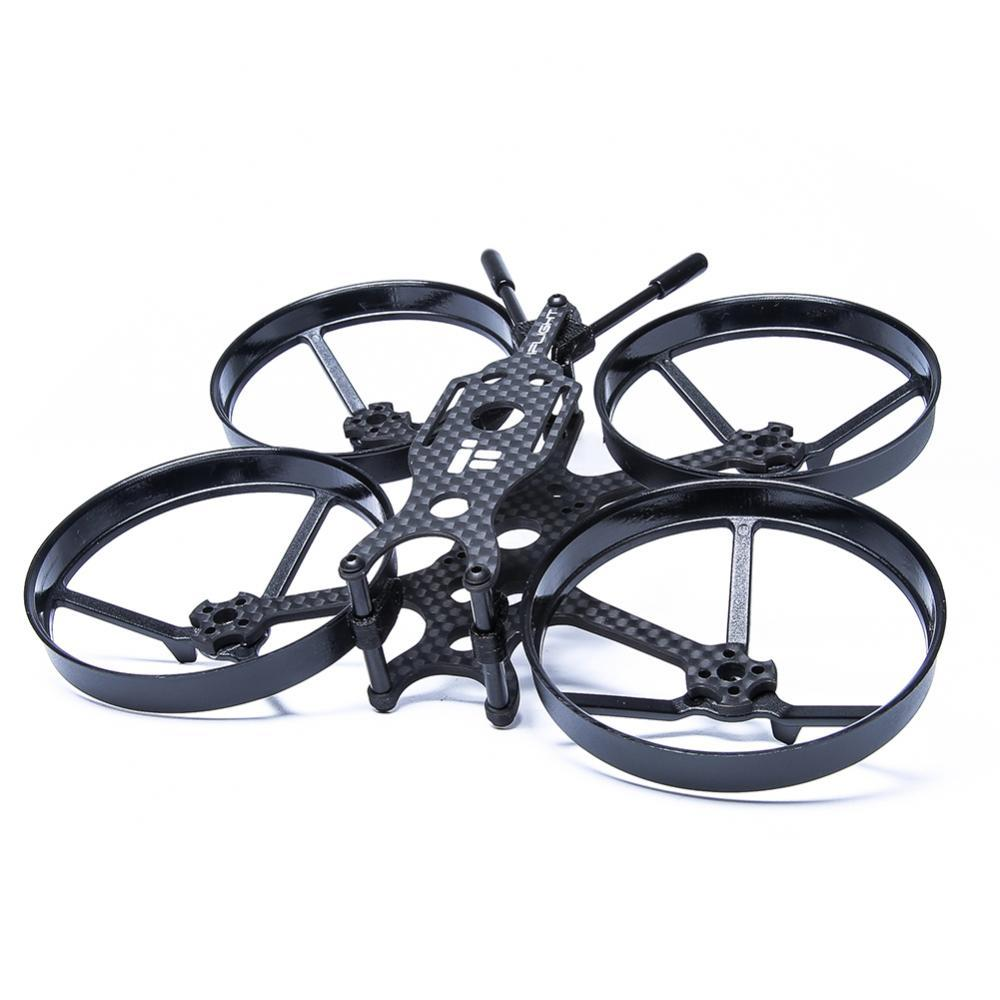
\includegraphics[width=0.5\linewidth]{../RW/pics/frame}
	\caption{Рама для экспериментального образца квадрокоптера
	}
	\label{fig:frame}
\end{figure}

Данная рама используется для создания экспериментального образца. В случае массового производства комплектов, которые будут получены при достижении поставленной цели, рама может быть заменена собственной разработкой.

Перейдем к выбору электроники.

Электроника квадрокоптера должна быть совместимой по характеристикам и габаритам. 

Для управления с наземной станции полетный контроллер должен:
\begin{itemize}
	\item обладать минимум 2 UART портами;
	\item быть совместимым с прошивкой PX4.
\end{itemize}

UART (Universal asynchronous receiver / transmitter) -- это аппаратный последовательный интерфейс, который позволяет подключать датчики и периферию к полетному контроллеру. У него есть два вывода для внешнего соединения: TX -- для передачи данных, RX -- для приема.

UART порты потребуются для подключения устройства приема -- передачи телеметрии и возможности подключения дополнительной периферии.

Выбор чипа процессора основан на требованиях к ресурсам по памяти, производительности и периферии. Для того, чтобы прошить PX4, необходим объем памяти процессора не ниже 1 МБ. Такое условие выполняют процессоры на базе F405 / F745 / F765. Преимущество F7 чипов в том, что обладают большими вычислительными способностями и ресурсами, но они дороже, выбор полетных контроллеров на таких чипах меньше, а разработка собственного полетного контроллера пока не целесообразна.
% дописать вставить таблицу https://ru.wikipedia.org/wiki/STM32

Винто-моторная группа должна быть оптимизирована под задачи автономного полета в помещении на небольшой скорости. Под такую задачу подходит низкооборотистая ВМГ с максимально большим диаметром пропеллера и минимально возможным шагом, что дает небольшую скорость полета и максимальную статическую тягу. Под выбранную раму походят пропеллеры диаметром 2-2.3". Проведен анализ рынка и выбраны пропеллеры с диаметром 2.3" и шагом 3.5". При одинаковых объемах статора мотора крутящий момент на низких оборотах будет больше у того мотора, где больше диаметр статора, а на высоких оборотах там, где больше высота. Для экспериментального образца оптимальным выбором являются моторы 1202. В четырехзначном числе маркировки мотора первые две цифры отвечают за диаметр статора, вторые -- за высоту. Количество оборотов на вольт (kv) выбирается, учитывая напряжение аккумулятора. Чем больше напряжение, тем меньше количество оборотов на вольт должно быть на моторе. Каждая ячейка, подключенная последовательно увеличивает напряжение на 4.2 В в заряженном состоянии. Для квадрокоптера с диагональю рамы 120 мм по соотношению вес / токоотдача наиболее выгодно ставить аккумуляторы с 2-3 ячейками. Основываясь на таблице характеристик, приведенных производителем, были выбраны моторы с 6000 kv (рисунок \ref{fig:motor}).
Учитывая потребление тока моторами на полном газу и добавляя 10 -- 15 \% запаса, получаем характеристику регуляторов -- максимальный ток, проходящий через них. На экспериментальном образце он равен 15 А.
\begin{figure}[H]
	\centering
	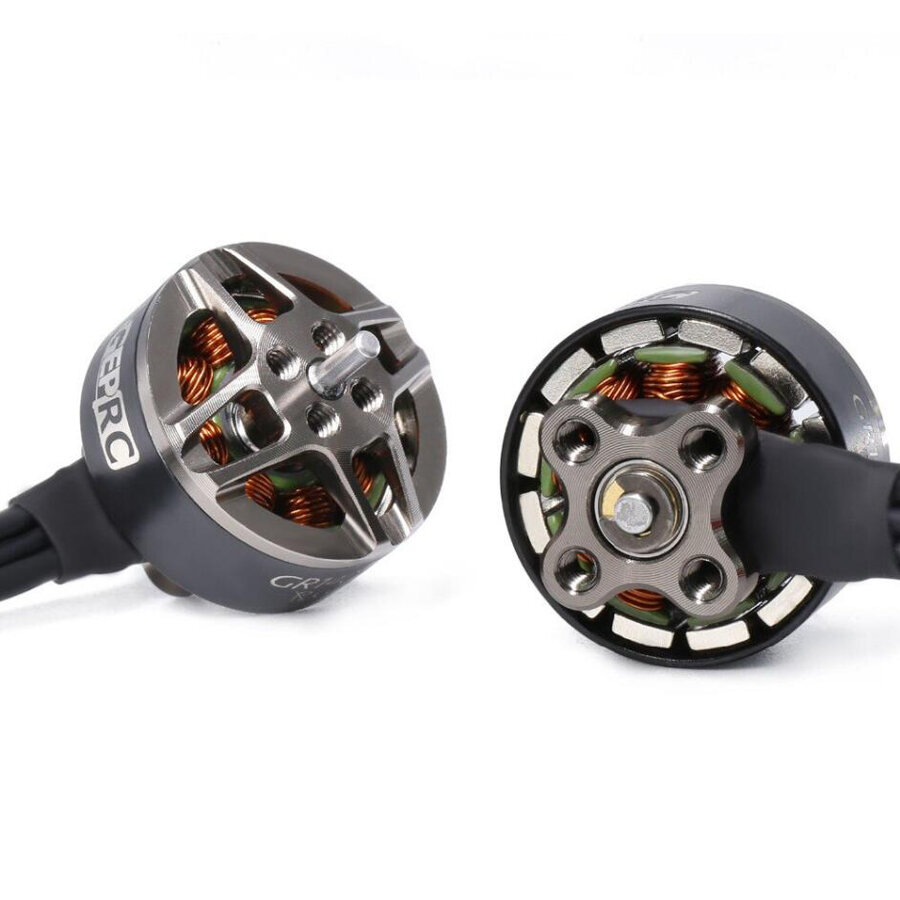
\includegraphics[width=0.5\linewidth]{../RW/pics/motor}
	\caption{Моторы для экспериментального образца квадрокоптера
	}
	\label{fig:motor} % эта метка позволяет ссылаться на рисунок в тексте
\end{figure}

\begin{figure}[H]
	\centering
	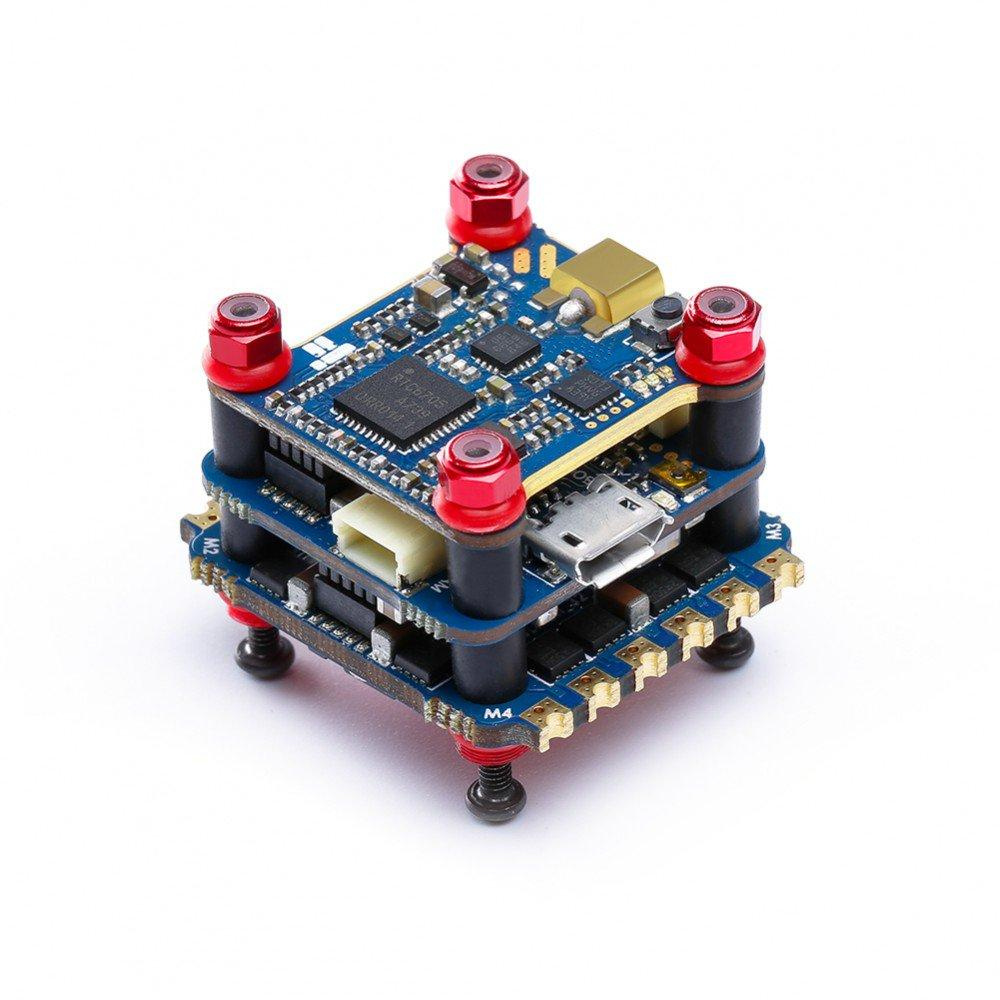
\includegraphics[width=0.5\linewidth]{../RW/pics/stack}
	\caption{Стек электроники для экспериментального образца квадрокоптера
	}
	\label{fig:stack} % эта метка позволяет ссылаться на рисунок в тексте
\end{figure}

Видеопередатчик и камера выбирались исходя из поставленных условий. Видеосигнал аналогового типа дешевле и передается с задержкой меньше, чем цифровой сигнал. MVP решение основывается на аналоговом сигнале. Так как необходимо будет передавать видеопоток, камера должна иметь максимально возможное количество телевизионных линий -- разрешающая способность (TVL). Для камер нано формата это 1000 TVL. Размер изображения может быть 4:3 и 16:9. Формат PAL / NTSC также может быть выбран на усмотрение.

Видеопередатчик обладает такими характеристиками как:
\begin{itemize}
	\item выходная мощность;
	\item выходная частота;
	\item количество каналов.
\end{itemize}

Для помещений нет необходимости использования высокой мощности видеопередачи, потому используется минимально возможная -- 25mW. Частота видеосигнала 5.8 ГГц.

Для общения с наземной станцией квадрокоптеру понадобятся устройства приема-передачи телеметрии. Протокол, бод-рейт (скорость передачи данных для подключенного устройства приема-передачи данных) и частота устройств станции и квадрокоптера должны совпадать. Для экспериментального образца были выбраны радиомодуль и приемник с поддержкой двусторонней телеметрии MavLink на частоте 2.4 ГГц.

Из указанных компонентов был собран дрон, результат представлен в отчете научно-исследовательской работы \cite{nir1}. В ходе тестирования была выявлена высокая задержка при получении видеосигнала. Такая задержка обусловлена суммой задержек каждого устройства (камеры, видеопередатчика, видеоприемника, USB порта компьютера). Учитывая, что задержка также присутствует на устройстве приема-передачи телеметрии, было необходимо провести исследование с использованием цифровой видеопередачи и сравнить результаты. В отчете научно-исследовательской работы \cite{nir2} представлен результат: задержка уменьшилась с 217 мс до 150 мс, а качество изображения значительно улучшилось.

%дописать по результатам работы не сошлось с ожиданием, потму было решено испольщрвать микрокомпьютер для трансляции видео такой то и он подключен туда то

На борт квадрокоптера был установлен микрокомпьютер RPi zero w со встроенным wifi-модулем. Стандартным шлейфом к интерфейсу CSI подключается камера размером 60*11.5*5 мм. Угол обзора камеры 72 градуса, разрешение 5 МП. Максимальное разрешение видео составляет 1080p. 

После настройки программной части полетного контроллера (прошивки) будет необходима подготовка образа и настройка окружения для трансляции видеопотока с борта дрона.


%\url{https://dev.px4.io/v1.9.0/en/ros/offboard\_control.html}
%\url{https://dev.px4.io/v1.9.0/en/ros/external_position_estimation.html}
\subsection{Настройка дрона для передачи телеметрии и видеопотока на наземную станцию}

%\https://discuss.ardupilot.org/t/indoor-autonomous-flight-with-arducopter-ros-and-aruco-boards-detection/34699

\subsubsection{Настройка PX4}
Через конфигуратор qgroundcontrol на полетный контроллер загружается прошивка PX4, после чего необходима первоначальная настройка.

Последовательность действий:
\begin{itemize}
	\item указание прошивке на тип и схему БПЛА (квадрокоптер);
	\item калибровку датчиков (акселерометра, магнитометра, гироскопа...);
	\item проверка корректности ориентации датчиков положения -- акселерометра и гироскопа (отклонения по всем осям происходят в нужные стороны);
	\item конфигурация протокола радиоуправления;
	\item калибровка и настройка каналов радиоуправления (выставлены последовательно соответствующие оси и добавлены необходимые режимы);
	\item проверяется и задается последовательность моторов (порядковые номера моторов соответствуют используемым прошивкой полетного контроллера);
	\item проверяется направление вращений моторов и пропеллеров (диагональные моторы вращаются в одинаковых направлениях согласно выбранной схеме ЛА).
\end{itemize}

Часто в связи с некорректной настройкой одного из описанных пунктов возникают неконтролируемые ситуации при старте -- дрон отказывается взлетать или переворачивается при взлете.

Выставляются полетные режимы:

ACRO -- режим, где отклонением стиков задается угловая скорость для соответствующей оси дрона. Центральное положение стика означает нулевую угловую скорость; в то время как угловая скорость при крайнем положении настраивается значением системы рейтов. Таким образом, при нулевом положении стика дрон не возвращается в горизонт (отсутствует стабилизация уровня). Режим ACRO используется для акробатических полетов, когда требуется плавное и быстрое управление \cite{ardupilot}.

STABILIZED -- режим стабилизации дрона, когда стики аппаратуры находятся в центре; используется для ручного управления в ходе полетных испытаний внутри помещения.

POSHOLD -- удержание позиции по датчикам / компьютерному зрению; когда будет настроена система оценки положения дрона в пространстве, при включении указанного режима дрон должен держаться в одной точке с учетом погрешности.

OFFBOARD -- управление полетом с внешнего компьютера. Этот режим используется для программирования автономных полетов \cite{clover}, при котором управление происходит из выполняемой на внешнем компьютере программы.

После выполнения описанных в начале раздела шагов производится взлет в ручных режимах. Во время полета проверяется ПИД регулирование.

Настройка ПИД-регулятора производится стандартным методом анализа реакции step res\-ponse \cite{tau}.
%дописать посмотреть метод в книге
Суть метода заключается в передаче ступенчатого управляющего сигнала на вход регулятора и анализе реакции системы на него.
Медленная реакция на ступенчатый управляющий сигнал указывает на низкий коэффициент пропорциональной составляющей.
Коэффициент увеличивается до появления характерного перерегулирования.
После чего остаточные осцилляции гасятся путем повышения коэффициента дифференциальной составляющей.

Далее изменяются параметры для взаимодействия с Raspberry Pi: указывается используемый порт (UART) и бод-рейт 921600.
Для уменьшения задержки вместо всех MavLink сообщений на наземную станцию будут отправляться только сообщения внешнего визуального позиционирования.
%по умолчанию мавлинк функционирует в режиме, где передает все имеющиеся сообщения, но это не нужно, так как вносится задержка. изначально планировалась кастомная сборка для отправки самых необходимых, но оказалось, что от разработчика есть выбор типа сообщений для отправки, и был определен тип, где выбраны только сообщения внешнего визуального позиционирования.
Программно отключаются использование компаса и GPS, так как они не устанавливаются на борт дрона, и выставляются параметры для оценки положения по EKF.

В качестве источника картинки для системы внешнего визуального позиционирования используется RPi c камерой.
% дописать RPi выполняет следующие функции. дальше написать для достижения выбрана ОС и тд
% В качестве для системы внешнего визуального позиционирования используется рос-среда
%https://docs.px4.io/master/en/advanced_config/tuning_the_ecl_ekf.html

%https://docs.px4.io/master/en/ros/external_position_estimation.html
%https://docs.px4.io/master/en/peripherals/mavlink_peripherals.html

\subsubsection{Настройка Raspberry Pi}

Для RPi выбрана операционная система raspbian stretch lite.
%http://www.pcds.fi/downloads/operatingsystem/debianbased/raspbian/archive/stretch/raspbian.stretch.html
С помощью команд, представленных в листинге \ref{lst:5}, был записан образ на карту памяти микрокомпьютера.
\begin{Program}[H]
	\caption{Подготовка карты памяти для RPi} \label{lst:5}
	\begin{MyCode}
	$ unzip -p 2018-11-13-raspbian-stretch-lite.zip
	$ sudo dd if=/home/qw/2018-11-13-raspbian-stretch-lite.img of=/dev/sdd
	$ sync
	\end{MyCode}
Для подключения к роутеру изменены параметры wpa\_supplicant.conf.

	\begin{MyCode}
	$ less /etc/wpa_supplicant/wpa_supplicant.conf
	ctrl_interface=DIR=/var/run/wpa_supplicant GROUP=netdev
	update_config=1
	country=RU
	
	network={
		ssid=<<ИМЯ_ТОЧКИ_ДОСТУПА>>
		psk=passwd
	}
		\end{MyCode}
\end{Program}

%https://habr.com/ru/post/419947/
Для того, чтобы на RPi активировать возможность удаленного подключения по протоколу ssh необходимо запустить сервис ssh. Это возможно % дописать 
создан файл ssh в каталоге /boot.
% дописать после проведенных шагов карта вставляется и для удаленного подключения необходимо просканировать сеть и найти адрес распбери
После произведенных шагов карта памяти устанавливается в RPi, и с помощью утилиты nmap на наземной станции проверяются все подключения к роутеру (листинг \ref{lst:6}).
\begin{Program}[H]
	\caption{Поиск адресов в подсети роутера} \label{lst:6}
	\begin{MyCode}
	$ sudo nmap -sn 192.168.1.0/24
	...
	Nmap scan report for 192.168.1.148
	Host is up (-0.062s latency).
	MAC Address: B8:27:EB:D3:B7:09 (Raspberry Pi Foundation)
	Nmap scan report for ikherty (192.168.1.28)
	Host is up.
	Nmap done: 256 IP addresses (4 hosts up) scanned in 4.42 seconds
	...
	\end{MyCode}
\end{Program}

192.168.1.148 -- ip-адрес Raspberry Pi, назначенный используемым роутером.

%https://www.raspberrypi.org/documentation/remote-access/ip-address.md
Производится удаленное подключение по ssh по найденному адресу, и устанавливаются пакеты gstreamer для запуска трансляции видео с борта дрона.
Для обмена данными между полетным контроллером и RPi устанавливается пакет ser2net и в конфигурационном файле /etc/ser2net.conf добавляется строка, определяющая способ общения, в данном случае она выглядит так (листинг \ref{lst:7}):
\begin{Program}[H]
\caption{Параметры для обмена сообщениями между полетным контроллером и RPi} \label{lst:7}
	\begin{MyCode}
	2000:raw:0:/dev/ttyAMA0:115200 8DATABITS NONE 1STOPBIT
	\end{MyCode}
\end{Program}

%дописать как работает и формат строки сер2нет
В случае с Raspberry источником видеопотока (element1) является rpi\-cam\-src, который захватывает изображение с RPi камеры. rpi\-cam\-src может выводить видео в виде необработанных кадров или закодированное в формате (M)JPEG или H.264 \cite{gstreamer1}. В качестве element2 будет выступать устройство вывода udpsink,-- это сетевой приемник, который отправляет UDP-пакеты в сеть.

Для использования RPi камеры в качестве источника данных трансляции производится сборка gst-rpicamsrc из репозитория \url{https://github.com/thaytan/gst-rpicamsrc} с помощью команд, представленных в листинге \ref{lst:8}:
\begin{Program}[H]
\caption{Сборка rpicamsrc} \label{lst:8}
	\begin{MyCode}
	$ git clone https://github.com/thaytan/gst-rpicamsrc
	$ cd gst-rpicamsrc
	$ make
	$ make install
	\end{MyCode}
\end{Program}


Все необходимые изменения внесены, далее следует произвести настройку наземной станции.

